\section{Objective}

The aim of this project is to create an application that retrieves photographed documents in an image where the document does not cover the full width and height of the image. It does so by utilising a perspective transformation. In figure \ref{fig:genius} shows an example of this. In the figure one can see an example of the app "Genius Scan" which recognises the edges of the document in red in a photographed image and transforms it to a full screen view.

\begin{figure}[H]
    \centering
    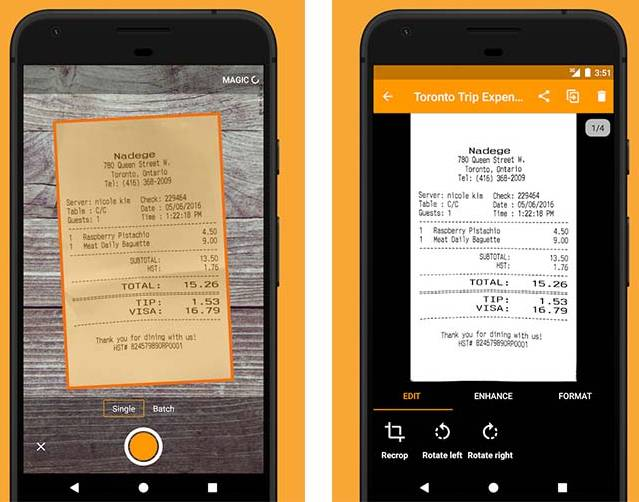
\includegraphics[width=.6\textwidth]{images/Genius-Scan-screenshot-2018.jpg}
    \caption{Example of the app Genius Scan\\Source: \citep{genius}}
    \label{fig:genius}
\end{figure}

To achieve the same results the algorithm has to fulfill the following tasks:
\begin{enumerate}
    \item Calculate the position of the four corner points
    \item Use a perspective transformation to get a clean top-view of the document
    \item Filter the scanned document to get a clear binary image
\end{enumerate}

\vspace{\lineskip}

Meanwhile the following basic properties of the image with the photographed document are assumed:
\begin{itemize}[leftmargin=0.9cm]
    \item Each document is an approximately rectangular object with four right-angled corners.
    \item Only one document is fully and clearly captured per image.
    \item There are text or figures on the document.
    \item The corners of the photographed document are clearly visible.
\end{itemize}


